\section{Crowd plugin development (WP4)}

\paragraph{Generation of the path}~

\noindent The algorithm of least-effort approach is divided in many points.
\begin{itemize}
  \item Computing an approxiamation graph to give an indication of the distance remaning to travel to the goal of the individual. We englobe the whole ground zone with a grid of a given mesh to reprensent this graph.
  \item Finding the exclusion zones that cannot be crossed by the individuals of the crowd. They will be given by a set of polygon that will be projet on the surface where the individual travel.
  \item Computation of the authorised velocity field that will be collinsion proof. This will be done by an approximation algorithm that will represent the field by an intersection of half-planes.
  \item Computation of the best velocity to choose by doing minimum on a graph with the $A*$ algorithm to approximate the remaning distance after traveling during dt at this velocity.
  \item Update of the graph with the attribution of a new weight on the edges: each character affect the weight of its neighbour edges to represent conjection. The way we will do this is still not fixed and will be decided by trying impericactly some ways.
\end{itemize}

\noindent We also started coding the classes that we will use (summarised on Figure \ref{crowd_classes}):
\begin{description}
  \item[Graph] This class describes the graph that was set up, with a set of nodes and a dictionary of dictionaries of edges.
  \item[Individual] This class describe an individual within the crowd. It includes the position, maximal speed, optimal speed, trajectory and some variables to compute the energy of the individual.
  \item[Crowd] contains a set of individuals and the graph.
  \item[Environment] gives the set of forbidden regions.
  \item[Blend*] These are the classes using Blender. They take the corresponding ``non-blend'' class and convert it into a Blender object, usable in Blender. 
\end{description}

We also try to keep as much code as possible independent from Blender. It will lead to easier tests and a more portable code from Blender to another 3D software.

\begin{figure}[h]
  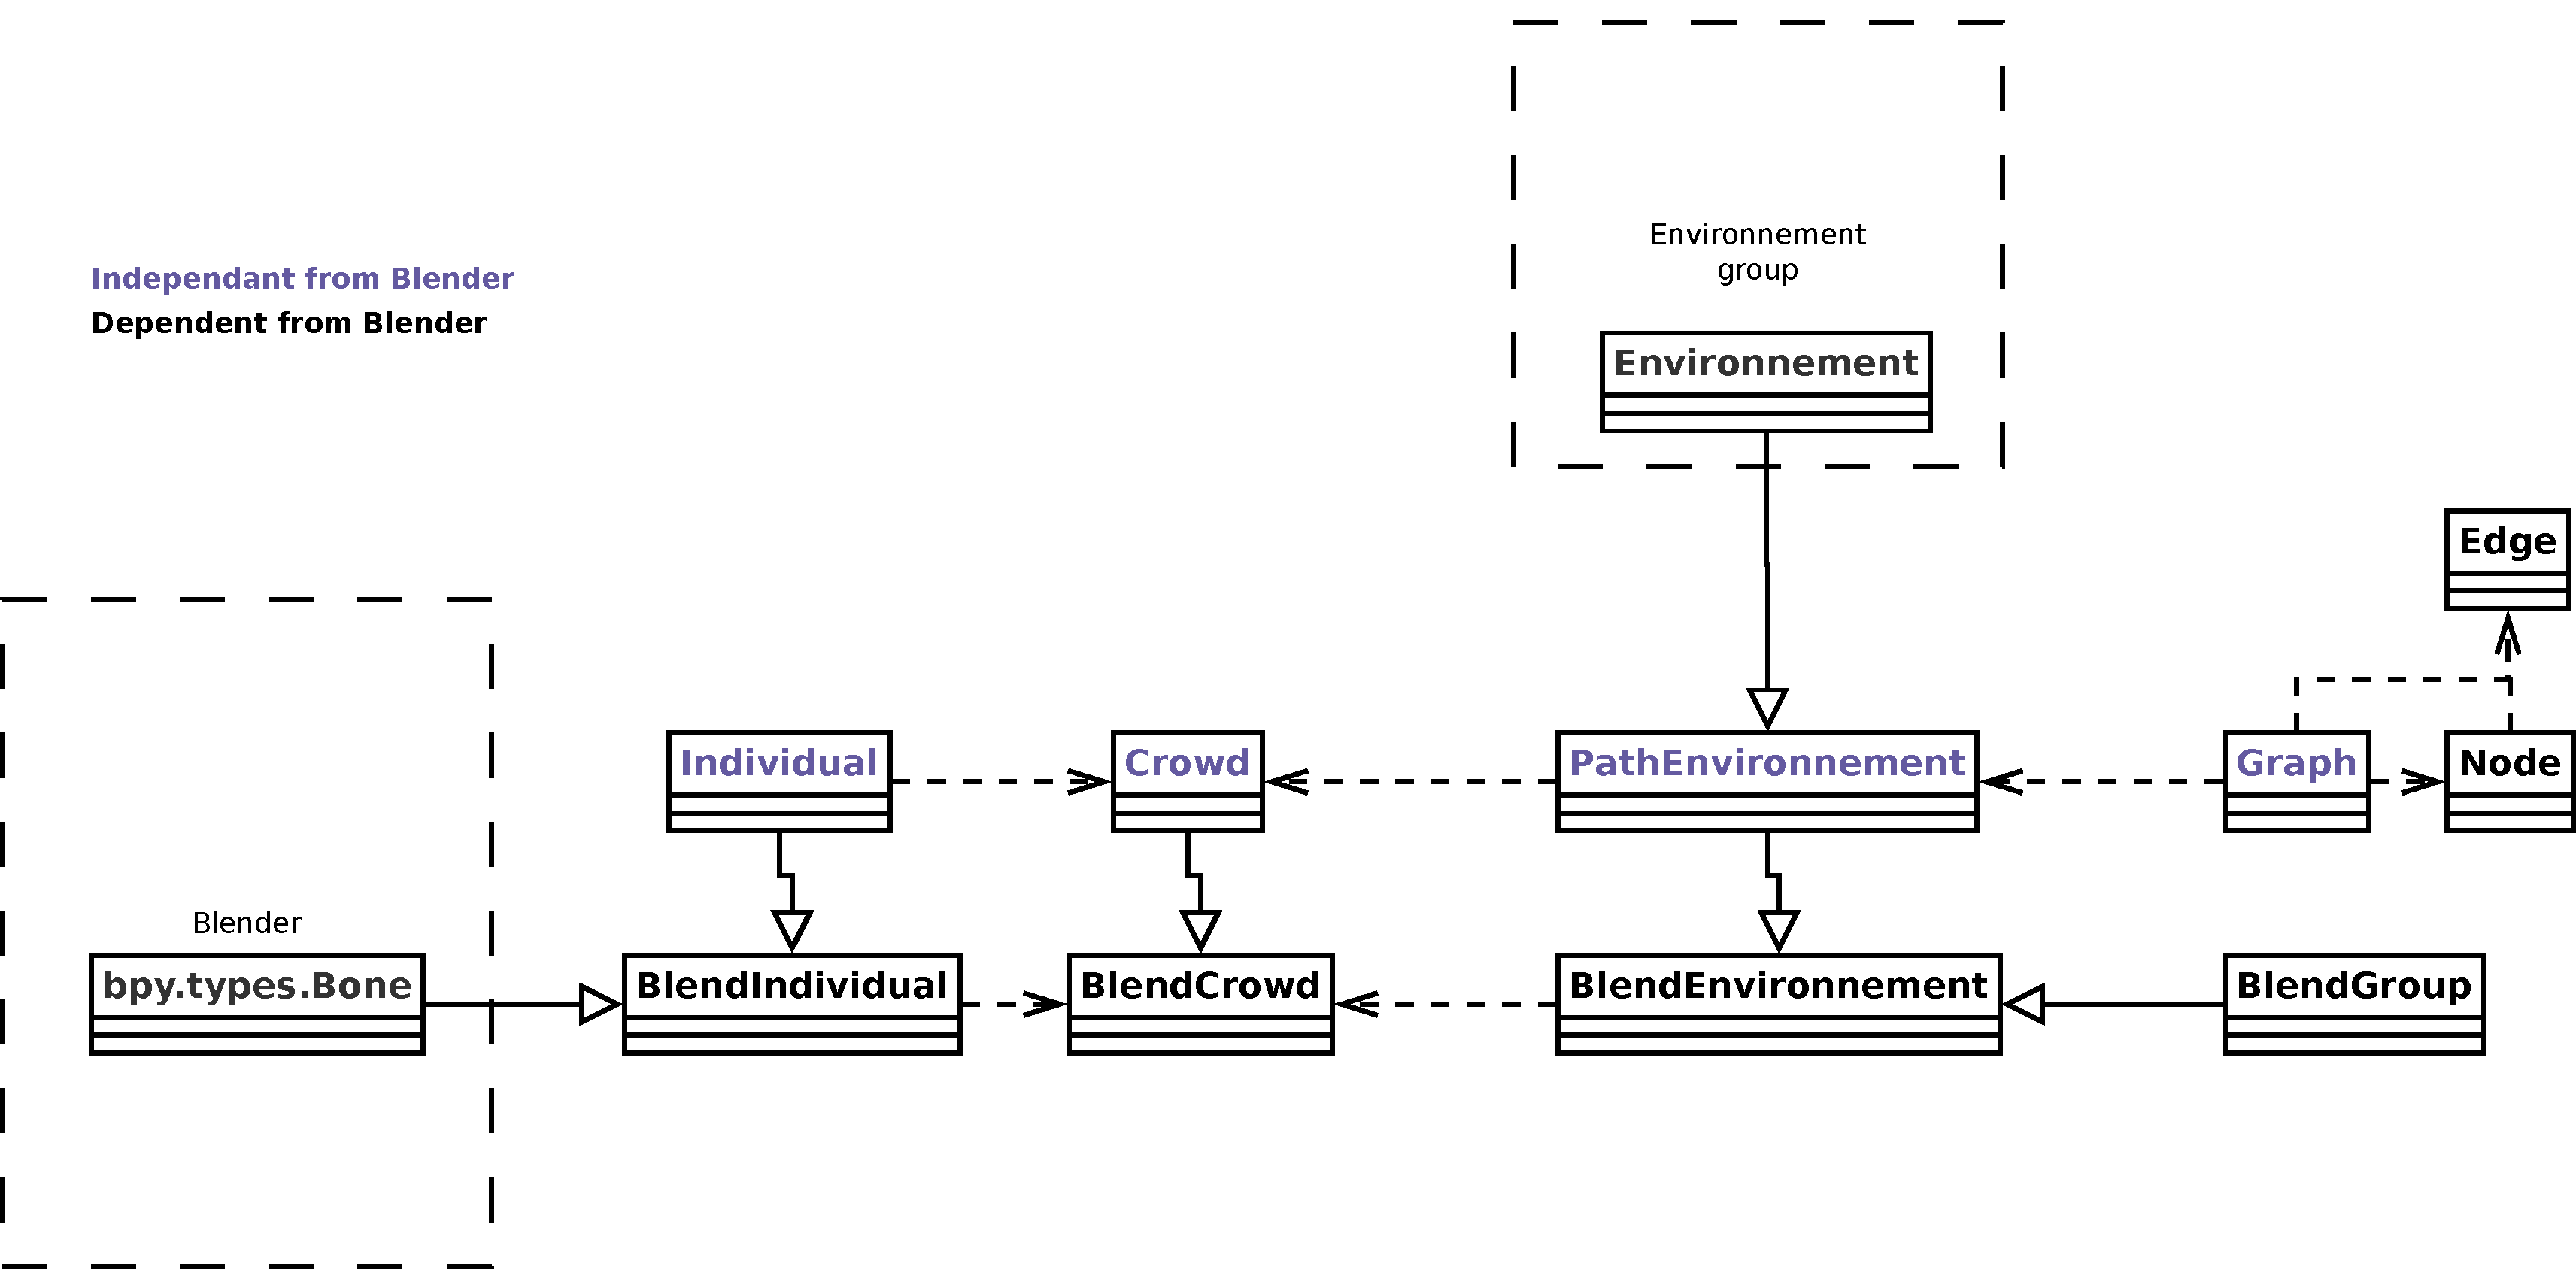
\includegraphics[width=15cm]{crowd_final.pdf}
  \caption{Classes of \texttt{crowd plug-in} and relations between them.}
  \label{crowd_classes}
\end{figure}

\paragraph{Motions of the characters}~

As stated in the paragraph \ref{WP2_motion}, the bibliographical work on the animation of characters was longer than expected and is currently being finalised: the implementation part has yet not begun.



